\documentclass[a4paper]{article}
\usepackage[a4paper,margin=1in,landscape]{geometry}
\usepackage[utf8]{inputenc}
\usepackage[T1]{fontenc}
\usepackage{longtable}
\usepackage[table,svgnames]{xcolor}
\usepackage{colortbl}
\usepackage{pgfplots}
\pgfplotsset{width=10cm,compat=1.14}
\usepgfplotslibrary{dateplot}
\usetikzlibrary{plotmarks}
\usepackage{booktabs}
\usepackage{array}
\usepackage{eurosym}
\usepackage{forest}
\usepackage{listings}
\usepackage{multicol}
\usepackage{fancyhdr}
\pagestyle{fancy}
\lfoot{Section \leftmark}
\cfoot{}
\rfoot{\thepage}
\rhead{Generated: \today}
\chead{}
\lhead{Scheduling Report}
\usepackage{hyperref}
\title{Scheduling Report}
\author{L. O'Toole and H. Simonis}
\date{Report Generated on \today}

\begin{document}
\maketitle
\definecolor{stagecolor0}{RGB}{240,163,255}
\definecolor{stagecolor1}{RGB}{0,117,220}
\definecolor{stagecolor2}{RGB}{153,63,0}
\definecolor{stagecolor3}{RGB}{76,0,92}
\definecolor{stagecolor4}{RGB}{25,25,25}
\definecolor{stagecolor5}{RGB}{0,92,49}
\definecolor{stagecolor6}{RGB}{43,206,72}
\definecolor{stagecolor7}{RGB}{255,204,153}
\section{Introduction}

\begin{table}[htbp]
\caption{Problem}
\centering
\begin{tabular}{lrrrrrrrr} \toprule
Name &\shortstack{Timepoints\\as\\Date} &\shortstack{Nr\\Products} &\shortstack{Nr\\Process} &\shortstack{Nr\\Disjunctive\\Resources} &\shortstack{Nr\\Cumulative\\Resources} &\shortstack{Nr\\Orders} &\shortstack{Nr\\Jobs} &\shortstack{Nr\\Tasks} \\ \midrule
P1&true&5&5&8&1&20&20&80\\ 
\bottomrule
\end{tabular}
\end{table}

\section{Orders}

\begin{longtable}{lllrrrrr}
\caption{Orders (Total 20)}
\\ \toprule
Name &Product &Process &Qty &Release &Due &Earliness Weight &Lateness Weight \\ \midrule
\endfirsthead
\toprule
Name &Product &Process &Qty &Release &Due &Earliness Weight &Lateness Weight \\ \midrule
\endhead
\bottomrule
\endfoot
Order0&Prod0&Process 0&2&0&973& 1.00& 1.00\\ 
Order1&Prod2&Process 2&2&0&2,243& 1.00& 1.00\\ 
Order2&Prod4&Process 4&4&0&928& 1.00& 1.00\\ 
Order3&Prod4&Process 4&1&0&2,546& 1.00& 1.00\\ 
Order4&Prod3&Process 3&1&0&2,809& 1.00& 1.00\\ 
Order5&Prod3&Process 3&4&0&506& 1.00& 1.00\\ 
Order6&Prod1&Process 1&5&0&800& 1.00& 1.00\\ 
Order7&Prod0&Process 0&7&0&159& 1.00& 1.00\\ 
Order8&Prod3&Process 3&5&0&2,759& 1.00& 1.00\\ 
Order9&Prod1&Process 1&5&0&1,852& 1.00& 1.00\\ 
Order10&Prod1&Process 1&2&0&287& 1.00& 1.00\\ 
Order11&Prod1&Process 1&4&0&80& 1.00& 1.00\\ 
Order12&Prod1&Process 1&8&0&1,696& 1.00& 1.00\\ 
Order13&Prod4&Process 4&4&0&1,838& 1.00& 1.00\\ 
Order14&Prod3&Process 3&5&0&2,542& 1.00& 1.00\\ 
Order15&Prod2&Process 2&5&0&1,013& 1.00& 1.00\\ 
Order16&Prod3&Process 3&2&0&1,602& 1.00& 1.00\\ 
Order17&Prod2&Process 2&5&0&2,862& 1.00& 1.00\\ 
Order18&Prod2&Process 2&6&0&335& 1.00& 1.00\\ 
Order19&Prod2&Process 2&9&0&2,403& 1.00& 1.00\\ 
\end{longtable}

\section{Solution}

\begin{table}[htbp]
\caption{Solutions (Total 1)}
\centering
\begin{tabular}{llrrrrrrrrrrrllr} \toprule
Name &\shortstack{Solver\\Status} &\shortstack{Objective\\Value} &Bound &Gap &Makespan &Flowtime &\shortstack{Total\\Lateness} &\shortstack{Max\\Lateness} &\shortstack{Nr\\Late} &\shortstack{Total\\Earliness} &\shortstack{Max\\Earliness} &\shortstack{Nr\\Early} &\shortstack{Model\\Type} &\shortstack{Objective\\Type} &Time \\ \midrule
Sol1&Solution&903&549.00& 0.39&903&13,188&1,823&786&4&18,868&2,430&16&CPO&Makespan&60.10\\ 
\bottomrule
\end{tabular}
\end{table}

\begin{figure}[htbp]
\caption{Machine Gantt for Solution Sol1}
\label{resourceGantt}
\centering
\begin{tikzpicture}[xscale=1.000000,yscale=1.000000]
\draw[draw=black!20] (0.000000,7.000000) -- (0.000000,-0.100000);
\node[below] at (0.000000,-0.100000) {0};
\draw[draw=black!20] (2.547065,7.000000) -- (2.547065,-0.100000);
\node[below] at (2.547065,-0.100000) {100};
\draw[draw=black!20] (5.094131,7.000000) -- (5.094131,-0.100000);
\node[below] at (5.094131,-0.100000) {200};
\draw[draw=black!20] (7.641196,7.000000) -- (7.641196,-0.100000);
\node[below] at (7.641196,-0.100000) {300};
\draw[draw=black!20] (10.188261,7.000000) -- (10.188261,-0.100000);
\node[below] at (10.188261,-0.100000) {400};
\draw[draw=black!20] (12.735327,7.000000) -- (12.735327,-0.100000);
\node[below] at (12.735327,-0.100000) {500};
\draw[draw=black!20] (15.282392,7.000000) -- (15.282392,-0.100000);
\node[below] at (15.282392,-0.100000) {600};
\draw[draw=black!20] (17.829457,7.000000) -- (17.829457,-0.100000);
\node[below] at (17.829457,-0.100000) {700};
\draw[draw=black!20] (20.376523,7.000000) -- (20.376523,-0.100000);
\node[below] at (20.376523,-0.100000) {800};
\draw[draw=black!20] (22.923588,7.000000) -- (22.923588,-0.100000);
\node[below] at (22.923588,-0.100000) {900};
\draw[draw=black!20] (0.000000,7.000000) -- (0.000000,-0.050000);
\draw[draw=black!20] (1.273533,7.000000) -- (1.273533,-0.050000);
\draw[draw=black!20] (2.547065,7.000000) -- (2.547065,-0.050000);
\draw[draw=black!20] (3.820598,7.000000) -- (3.820598,-0.050000);
\draw[draw=black!20] (5.094131,7.000000) -- (5.094131,-0.050000);
\draw[draw=black!20] (6.367663,7.000000) -- (6.367663,-0.050000);
\draw[draw=black!20] (7.641196,7.000000) -- (7.641196,-0.050000);
\draw[draw=black!20] (8.914729,7.000000) -- (8.914729,-0.050000);
\draw[draw=black!20] (10.188261,7.000000) -- (10.188261,-0.050000);
\draw[draw=black!20] (11.461794,7.000000) -- (11.461794,-0.050000);
\draw[draw=black!20] (12.735327,7.000000) -- (12.735327,-0.050000);
\draw[draw=black!20] (14.008859,7.000000) -- (14.008859,-0.050000);
\draw[draw=black!20] (15.282392,7.000000) -- (15.282392,-0.050000);
\draw[draw=black!20] (16.555925,7.000000) -- (16.555925,-0.050000);
\draw[draw=black!20] (17.829457,7.000000) -- (17.829457,-0.050000);
\draw[draw=black!20] (19.102990,7.000000) -- (19.102990,-0.050000);
\draw[draw=black!20] (20.376523,7.000000) -- (20.376523,-0.050000);
\draw[draw=black!20] (21.650055,7.000000) -- (21.650055,-0.050000);
\draw[draw=black!20] (22.923588,7.000000) -- (22.923588,-0.050000);
\draw[draw=black!20] (24.197121,7.000000) -- (24.197121,-0.050000);
\node[draw=black,fill=blue!10,font=\scriptsize,minimum height=0.700000cm,above left] (DR7) at (0,0.000000) {DR7};
\node[draw=black,fill=blue!10,font=\scriptsize,minimum height=0.700000cm,above left] (DR6) at (0,0.875000) {DR6};
\node[draw=black,fill=blue!10,font=\scriptsize,minimum height=0.700000cm,above left] (DR5) at (0,1.750000) {DR5};
\node[draw=black,fill=blue!10,font=\scriptsize,minimum height=0.700000cm,above left] (DR4) at (0,2.625000) {DR4};
\node[draw=black,fill=blue!10,font=\scriptsize,minimum height=0.700000cm,above left] (DR3) at (0,3.500000) {DR3};
\node[draw=black,fill=blue!10,font=\scriptsize,minimum height=0.700000cm,above left] (DR2) at (0,4.375000) {DR2};
\node[draw=black,fill=blue!10,font=\scriptsize,minimum height=0.700000cm,above left] (DR1) at (0,5.250000) {DR1};
\node[draw=black,fill=blue!10,font=\scriptsize,minimum height=0.700000cm,above left] (DR0) at (0,6.125000) {DR0};
\draw[draw=black,fill=stagecolor0!10] (3.209302,6.125000) rectangle node {} (4.100775,6.825000);
\draw[draw=black,fill=stagecolor1!10] (4.508306,3.500000) rectangle node {} (5.043189,4.200000);
\draw[draw=black,fill=stagecolor2!10] (5.629014,1.750000) rectangle node {} (6.775194,2.450000);
\draw[draw=black,fill=stagecolor3!10] (6.775194,0.000000) rectangle node {} (7.539313,0.700000);
\draw[draw=black,fill=stagecolor0!10] (15.333333,6.125000) rectangle node {} (16.581395,6.825000);
\draw[draw=black,fill=stagecolor1!10] (18.669989,3.500000) rectangle node {} (19.612403,4.200000);
\draw[draw=black,fill=stagecolor2!10] (20.758583,1.750000) rectangle node {} (21.726467,2.450000);
\draw[draw=black,fill=stagecolor3!10] (21.828350,0.000000) rectangle node {} (22.643411,0.700000);
\draw[draw=black,fill=stagecolor0!10] (6.495017,5.250000) rectangle node {} (7.870432,5.950000);
\draw[draw=black,fill=stagecolor1!10] (7.921373,3.500000) rectangle node {} (9.704319,4.200000);
\draw[draw=black,fill=stagecolor2!10] (10.544850,1.750000) rectangle node {} (12.480620,2.450000);
\draw[draw=black,fill=stagecolor3!10] (12.888151,0.000000) rectangle node {} (13.957918,0.700000);
\draw[draw=black,fill=stagecolor0!10] (17.498339,6.125000) rectangle node {} (18.186047,6.825000);
\draw[draw=black,fill=stagecolor1!10] (19.612403,3.500000) rectangle node {} (20.401993,4.200000);
\draw[draw=black,fill=stagecolor2!10] (21.726467,1.750000) rectangle node {} (22.516058,2.450000);
\draw[draw=black,fill=stagecolor3!10] (22.541528,0.875000) rectangle node {} (23.000000,1.575000);
\draw[draw=black,fill=stagecolor0!10] (15.307863,5.250000) rectangle node {} (15.995570,5.950000);
\draw[draw=black,fill=stagecolor1!10] (20.401993,3.500000) rectangle node {} (20.885936,4.200000);
\draw[draw=black,fill=stagecolor2!10] (21.828350,2.625000) rectangle node {} (22.617940,3.325000);
\draw[draw=black,fill=stagecolor3!10] (22.643411,0.000000) rectangle node {} (22.974529,0.700000);
\draw[draw=black,fill=stagecolor0!10] (0.000000,5.250000) rectangle node {} (1.375415,5.950000);
\draw[draw=black,fill=stagecolor1!10] (1.375415,4.375000) rectangle node {} (2.470653,5.075000);
\draw[draw=black,fill=stagecolor2!10] (2.470653,2.625000) rectangle node {} (4.712071,3.325000);
\draw[draw=black,fill=stagecolor3!10] (8.379845,0.875000) rectangle node {} (9.169435,1.575000);
\draw[draw=black,fill=stagecolor0!10] (8.023256,6.125000) rectangle node {} (9.755260,6.825000);
\draw[draw=black,fill=stagecolor1!10] (9.755260,3.500000) rectangle node {} (12.429679,4.200000);
\draw[draw=black,fill=stagecolor2!10] (13.346622,1.750000) rectangle node {} (15.053156,2.450000);
\draw[draw=black,fill=stagecolor3!10] (15.053156,0.875000) rectangle node {} (16.836102,1.575000);
\draw[draw=red,fill=stagecolor0!10] (3.947951,5.250000) rectangle node {} (6.495017,5.950000);
\draw[draw=red,fill=stagecolor1!10] (6.495017,3.500000) rectangle node {} (7.921373,4.200000);
\draw[draw=red,fill=stagecolor2!10] (7.921373,2.625000) rectangle node {} (11.232558,3.325000);
\draw[draw=red,fill=stagecolor3!10] (11.232558,0.000000) rectangle node {} (12.888151,0.700000);
\draw[draw=black,fill=stagecolor0!10] (1.604651,6.125000) rectangle node {} (3.209302,6.825000);
\draw[draw=black,fill=stagecolor1!10] (3.209302,3.500000) rectangle node {} (4.508306,4.200000);
\draw[draw=black,fill=stagecolor2!10] (4.712071,2.625000) rectangle node {} (7.437431,3.325000);
\draw[draw=black,fill=stagecolor3!10] (7.437431,0.875000) rectangle node {} (8.379845,1.575000);
\draw[draw=black,fill=stagecolor0!10] (9.755260,6.125000) rectangle node {} (11.487265,6.825000);
\draw[draw=black,fill=stagecolor1!10] (12.404208,4.375000) rectangle node {} (15.078627,5.075000);
\draw[draw=black,fill=stagecolor2!10] (15.078627,1.750000) rectangle node {} (16.785161,2.450000);
\draw[draw=black,fill=stagecolor3!10] (16.836102,0.875000) rectangle node {} (18.619048,1.575000);
\draw[draw=red,fill=stagecolor0!10] (7.870432,5.250000) rectangle node {} (8.761905,5.950000);
\draw[draw=red,fill=stagecolor1!10] (11.105205,4.375000) rectangle node {} (12.404208,5.075000);
\draw[draw=red,fill=stagecolor2!10] (12.480620,1.750000) rectangle node {} (13.346622,2.450000);
\draw[draw=red,fill=stagecolor3!10] (13.346622,0.875000) rectangle node {} (14.289037,1.575000);
\draw[draw=red,fill=stagecolor0!10] (13.881506,6.125000) rectangle node {} (15.333333,6.825000);
\draw[draw=red,fill=stagecolor1!10] (16.454042,3.500000) rectangle node {} (18.669989,4.200000);
\draw[draw=red,fill=stagecolor2!10] (19.128461,2.625000) rectangle node {} (20.554817,3.325000);
\draw[draw=red,fill=stagecolor3!10] (20.554817,0.875000) rectangle node {} (22.057586,1.575000);
\draw[draw=black,fill=stagecolor0!10] (1.375415,5.250000) rectangle node {} (3.947951,5.950000);
\draw[draw=black,fill=stagecolor1!10] (3.947951,4.375000) rectangle node {} (7.997785,5.075000);
\draw[draw=black,fill=stagecolor2!10] (7.997785,1.750000) rectangle node {} (10.544850,2.450000);
\draw[draw=black,fill=stagecolor3!10] (10.544850,0.875000) rectangle node {} (13.168328,1.575000);
\draw[draw=black,fill=stagecolor0!10] (13.932447,5.250000) rectangle node {} (15.307863,5.950000);
\draw[draw=black,fill=stagecolor1!10] (16.937984,4.375000) rectangle node {} (18.720930,5.075000);
\draw[draw=black,fill=stagecolor2!10] (18.822813,1.750000) rectangle node {} (20.758583,2.450000);
\draw[draw=black,fill=stagecolor3!10] (20.758583,0.000000) rectangle node {} (21.828350,0.700000);
\draw[draw=black,fill=stagecolor0!10] (0.000000,6.125000) rectangle node {} (1.604651,6.825000);
\draw[draw=black,fill=stagecolor1!10] (1.604651,3.500000) rectangle node {} (2.903654,4.200000);
\draw[draw=black,fill=stagecolor2!10] (2.903654,1.750000) rectangle node {} (5.629014,2.450000);
\draw[draw=black,fill=stagecolor3!10] (7.539313,0.000000) rectangle node {} (8.481728,0.700000);
\draw[draw=black,fill=stagecolor0!10] (11.487265,6.125000) rectangle node {} (13.881506,6.825000);
\draw[draw=black,fill=stagecolor1!10] (15.078627,4.375000) rectangle node {} (16.937984,5.075000);
\draw[draw=black,fill=stagecolor2!10] (17.090808,2.625000) rectangle node {} (19.128461,3.325000);
\draw[draw=black,fill=stagecolor3!10] (19.128461,0.000000) rectangle node {} (20.707641,0.700000);
\draw[draw=black,fill=stagecolor0!10] (16.581395,6.125000) rectangle node {} (17.498339,6.825000);
\draw[draw=black,fill=stagecolor1!10] (18.720930,4.375000) rectangle node {} (19.408638,5.075000);
\draw[draw=black,fill=stagecolor2!10] (20.554817,2.625000) rectangle node {} (21.828350,3.325000);
\draw[draw=black,fill=stagecolor3!10] (22.057586,0.875000) rectangle node {} (22.541528,1.575000);
\draw[draw=black,fill=stagecolor0!10] (11.538206,5.250000) rectangle node {} (13.932447,5.950000);
\draw[draw=black,fill=stagecolor1!10] (14.594684,3.500000) rectangle node {} (16.454042,4.200000);
\draw[draw=black,fill=stagecolor2!10] (16.785161,1.750000) rectangle node {} (18.822813,2.450000);
\draw[draw=black,fill=stagecolor3!10] (18.822813,0.875000) rectangle node {} (20.401993,1.575000);
\draw[draw=red,fill=stagecolor0!10] (8.761905,5.250000) rectangle node {} (11.538206,5.950000);
\draw[draw=red,fill=stagecolor1!10] (12.429679,3.500000) rectangle node {} (14.594684,4.200000);
\draw[draw=red,fill=stagecolor2!10] (14.696567,2.625000) rectangle node {} (17.090808,3.325000);
\draw[draw=red,fill=stagecolor3!10] (17.294574,0.000000) rectangle node {} (19.128461,0.700000);
\draw[draw=black,fill=stagecolor0!10] (4.100775,6.125000) rectangle node {} (8.023256,6.825000);
\draw[draw=black,fill=stagecolor1!10] (8.023256,4.375000) rectangle node {} (11.105205,5.075000);
\draw[draw=black,fill=stagecolor2!10] (11.232558,2.625000) rectangle node {} (14.696567,3.325000);
\draw[draw=black,fill=stagecolor3!10] (14.696567,0.000000) rectangle node {} (17.294574,0.700000);
\draw[draw=red,thick] (23.000000,7.000000) -- (23.000000,0.000000);
\node[above left,font=\scriptsize] () at (23.000000,7.000000) {Cmax: 903};
\node[left,] () at (3.000000,-1.000000) {Stage0};
\node[right,draw=black,fill=stagecolor0!10,font=\scriptsize] () at (3.000000,-1.000000) {};
\node[left,] () at (5.000000,-1.000000) {Stage1};
\node[right,draw=black,fill=stagecolor1!10,font=\scriptsize] () at (5.000000,-1.000000) {};
\node[left,] () at (7.000000,-1.000000) {Stage2};
\node[right,draw=black,fill=stagecolor2!10,font=\scriptsize] () at (7.000000,-1.000000) {};
\node[left,] () at (9.000000,-1.000000) {Stage3};
\node[right,draw=black,fill=stagecolor3!10,font=\scriptsize] () at (9.000000,-1.000000) {};
\node[left,] () at (11.000000,-1.000000) {Late};
\node[right,draw=red,font=\scriptsize] () at (11.000000,-1.000000) {};
\end{tikzpicture}
\end{figure}
\begin{figure}[htbp]
\caption{Job Gantt for Solution Sol1}
\label{jobGantt}
\centering
\begin{tikzpicture}[xscale=1.000000,yscale=1.000000]
\draw[draw=black!20] (0.000000,13.000000) -- (0.000000,-0.100000);
\node[below] at (0.000000,-0.100000) {0};
\draw[draw=black!20] (2.547065,13.000000) -- (2.547065,-0.100000);
\node[below] at (2.547065,-0.100000) {100};
\draw[draw=black!20] (5.094131,13.000000) -- (5.094131,-0.100000);
\node[below] at (5.094131,-0.100000) {200};
\draw[draw=black!20] (7.641196,13.000000) -- (7.641196,-0.100000);
\node[below] at (7.641196,-0.100000) {300};
\draw[draw=black!20] (10.188261,13.000000) -- (10.188261,-0.100000);
\node[below] at (10.188261,-0.100000) {400};
\draw[draw=black!20] (12.735327,13.000000) -- (12.735327,-0.100000);
\node[below] at (12.735327,-0.100000) {500};
\draw[draw=black!20] (15.282392,13.000000) -- (15.282392,-0.100000);
\node[below] at (15.282392,-0.100000) {600};
\draw[draw=black!20] (17.829457,13.000000) -- (17.829457,-0.100000);
\node[below] at (17.829457,-0.100000) {700};
\draw[draw=black!20] (20.376523,13.000000) -- (20.376523,-0.100000);
\node[below] at (20.376523,-0.100000) {800};
\draw[draw=black!20] (22.923588,13.000000) -- (22.923588,-0.100000);
\node[below] at (22.923588,-0.100000) {900};
\draw[draw=black!20] (0.000000,13.000000) -- (0.000000,-0.050000);
\draw[draw=black!20] (1.273533,13.000000) -- (1.273533,-0.050000);
\draw[draw=black!20] (2.547065,13.000000) -- (2.547065,-0.050000);
\draw[draw=black!20] (3.820598,13.000000) -- (3.820598,-0.050000);
\draw[draw=black!20] (5.094131,13.000000) -- (5.094131,-0.050000);
\draw[draw=black!20] (6.367663,13.000000) -- (6.367663,-0.050000);
\draw[draw=black!20] (7.641196,13.000000) -- (7.641196,-0.050000);
\draw[draw=black!20] (8.914729,13.000000) -- (8.914729,-0.050000);
\draw[draw=black!20] (10.188261,13.000000) -- (10.188261,-0.050000);
\draw[draw=black!20] (11.461794,13.000000) -- (11.461794,-0.050000);
\draw[draw=black!20] (12.735327,13.000000) -- (12.735327,-0.050000);
\draw[draw=black!20] (14.008859,13.000000) -- (14.008859,-0.050000);
\draw[draw=black!20] (15.282392,13.000000) -- (15.282392,-0.050000);
\draw[draw=black!20] (16.555925,13.000000) -- (16.555925,-0.050000);
\draw[draw=black!20] (17.829457,13.000000) -- (17.829457,-0.050000);
\draw[draw=black!20] (19.102990,13.000000) -- (19.102990,-0.050000);
\draw[draw=black!20] (20.376523,13.000000) -- (20.376523,-0.050000);
\draw[draw=black!20] (21.650055,13.000000) -- (21.650055,-0.050000);
\draw[draw=black!20] (22.923588,13.000000) -- (22.923588,-0.050000);
\draw[draw=black!20] (24.197121,13.000000) -- (24.197121,-0.050000);
\node[draw=black,fill=green!10,font=\scriptsize,minimum height=0.520000cm,above left] (J3) at (0,0.000000) {J3};
\node[draw=black,fill=green!10,font=\scriptsize,minimum height=0.520000cm,above left] (J16) at (0,0.650000) {J16};
\node[draw=black,fill=green!10,font=\scriptsize,minimum height=0.520000cm,above left] (J1) at (0,1.300000) {J1};
\node[draw=black,fill=green!10,font=\scriptsize,minimum height=0.520000cm,above left] (J4) at (0,1.950000) {J4};
\node[draw=black,fill=green!10,font=\scriptsize,minimum height=0.520000cm,above left] (J13) at (0,2.600000) {J13};
\node[draw=black,fill=green!10,font=\scriptsize,minimum height=0.520000cm,above left] (J11) at (0,3.250000) {J11};
\node[draw=black,fill=green!10,font=\scriptsize,minimum height=0.520000cm,above left] (J17) at (0,3.900000) {J17};
\node[draw=black,fill=green!10,font=\scriptsize,minimum height=0.520000cm,above left] (J15) at (0,4.550000) {J15};
\node[draw=black,fill=green!10,font=\scriptsize,minimum height=0.520000cm,above left] (J9) at (0,5.200000) {J9};
\node[draw=black,fill=green!10,font=\scriptsize,minimum height=0.520000cm,above left] (J18) at (0,5.850000) {J18};
\node[draw=black,fill=green!10,font=\scriptsize,minimum height=0.520000cm,above left] (J6) at (0,6.500000) {J6};
\node[draw=black,fill=green!10,font=\scriptsize,minimum height=0.520000cm,above left] (J10) at (0,7.150000) {J10};
\node[draw=black,fill=green!10,font=\scriptsize,minimum height=0.520000cm,above left] (J2) at (0,7.800000) {J2};
\node[draw=black,fill=green!10,font=\scriptsize,minimum height=0.520000cm,above left] (J19) at (0,8.450000) {J19};
\node[draw=black,fill=green!10,font=\scriptsize,minimum height=0.520000cm,above left] (J7) at (0,9.100000) {J7};
\node[draw=black,fill=green!10,font=\scriptsize,minimum height=0.520000cm,above left] (J0) at (0,9.750000) {J0};
\node[draw=black,fill=green!10,font=\scriptsize,minimum height=0.520000cm,above left] (J8) at (0,10.400000) {J8};
\node[draw=black,fill=green!10,font=\scriptsize,minimum height=0.520000cm,above left] (J12) at (0,11.050000) {J12};
\node[draw=black,fill=green!10,font=\scriptsize,minimum height=0.520000cm,above left] (J14) at (0,11.700000) {J14};
\node[draw=black,fill=green!10,font=\scriptsize,minimum height=0.520000cm,above left] (J5) at (0,12.350000) {J5};
\draw[draw=black,fill=stagecolor0!10] (3.209302,9.750000) rectangle node {} (4.100775,10.270000);
\draw[draw=black,fill=stagecolor1!10] (4.508306,9.750000) rectangle node {} (5.043189,10.270000);
\draw[draw=black,fill=stagecolor2!10] (5.629014,9.750000) rectangle node {} (6.775194,10.270000);
\draw[draw=black,fill=stagecolor3!10] (6.775194,9.750000) rectangle node {} (7.539313,10.270000);
\draw[draw=black,fill=stagecolor0!10] (15.333333,1.300000) rectangle node {} (16.581395,1.820000);
\draw[draw=black,fill=stagecolor1!10] (18.669989,1.300000) rectangle node {} (19.612403,1.820000);
\draw[draw=black,fill=stagecolor2!10] (20.758583,1.300000) rectangle node {} (21.726467,1.820000);
\draw[draw=black,fill=stagecolor3!10] (21.828350,1.300000) rectangle node {} (22.643411,1.820000);
\draw[draw=black,fill=stagecolor0!10] (6.495017,7.800000) rectangle node {} (7.870432,8.320000);
\draw[draw=black,fill=stagecolor1!10] (7.921373,7.800000) rectangle node {} (9.704319,8.320000);
\draw[draw=black,fill=stagecolor2!10] (10.544850,7.800000) rectangle node {} (12.480620,8.320000);
\draw[draw=black,fill=stagecolor3!10] (12.888151,7.800000) rectangle node {} (13.957918,8.320000);
\draw[draw=black,fill=stagecolor0!10] (17.498339,0.000000) rectangle node {} (18.186047,0.520000);
\draw[draw=black,fill=stagecolor1!10] (19.612403,0.000000) rectangle node {} (20.401993,0.520000);
\draw[draw=black,fill=stagecolor2!10] (21.726467,0.000000) rectangle node {} (22.516058,0.520000);
\draw[draw=black,fill=stagecolor3!10] (22.541528,0.000000) rectangle node {} (23.000000,0.520000);
\draw[draw=black,fill=stagecolor0!10] (15.307863,1.950000) rectangle node {} (15.995570,2.470000);
\draw[draw=black,fill=stagecolor1!10] (20.401993,1.950000) rectangle node {} (20.885936,2.470000);
\draw[draw=black,fill=stagecolor2!10] (21.828350,1.950000) rectangle node {} (22.617940,2.470000);
\draw[draw=black,fill=stagecolor3!10] (22.643411,1.950000) rectangle node {} (22.974529,2.470000);
\draw[draw=black,fill=stagecolor0!10] (0.000000,12.350000) rectangle node {} (1.375415,12.870000);
\draw[draw=black,fill=stagecolor1!10] (1.375415,12.350000) rectangle node {} (2.470653,12.870000);
\draw[draw=black,fill=stagecolor2!10] (2.470653,12.350000) rectangle node {} (4.712071,12.870000);
\draw[draw=black,fill=stagecolor3!10] (8.379845,12.350000) rectangle node {} (9.169435,12.870000);
\draw[draw=black,fill=stagecolor0!10] (8.023256,6.500000) rectangle node {} (9.755260,7.020000);
\draw[draw=black,fill=stagecolor1!10] (9.755260,6.500000) rectangle node {} (12.429679,7.020000);
\draw[draw=black,fill=stagecolor2!10] (13.346622,6.500000) rectangle node {} (15.053156,7.020000);
\draw[draw=black,fill=stagecolor3!10] (15.053156,6.500000) rectangle node {} (16.836102,7.020000);
\draw[draw=red,fill=stagecolor0!10] (3.947951,9.100000) rectangle node {} (6.495017,9.620000);
\draw[draw=red,fill=stagecolor1!10] (6.495017,9.100000) rectangle node {} (7.921373,9.620000);
\draw[draw=red,fill=stagecolor2!10] (7.921373,9.100000) rectangle node {} (11.232558,9.620000);
\draw[draw=red,fill=stagecolor3!10] (11.232558,9.100000) rectangle node {} (12.888151,9.620000);
\draw[draw=black,fill=stagecolor0!10] (1.604651,10.400000) rectangle node {} (3.209302,10.920000);
\draw[draw=black,fill=stagecolor1!10] (3.209302,10.400000) rectangle node {} (4.508306,10.920000);
\draw[draw=black,fill=stagecolor2!10] (4.712071,10.400000) rectangle node {} (7.437431,10.920000);
\draw[draw=black,fill=stagecolor3!10] (7.437431,10.400000) rectangle node {} (8.379845,10.920000);
\draw[draw=black,fill=stagecolor0!10] (9.755260,5.200000) rectangle node {} (11.487265,5.720000);
\draw[draw=black,fill=stagecolor1!10] (12.404208,5.200000) rectangle node {} (15.078627,5.720000);
\draw[draw=black,fill=stagecolor2!10] (15.078627,5.200000) rectangle node {} (16.785161,5.720000);
\draw[draw=black,fill=stagecolor3!10] (16.836102,5.200000) rectangle node {} (18.619048,5.720000);
\draw[draw=red,fill=stagecolor0!10] (7.870432,7.150000) rectangle node {} (8.761905,7.670000);
\draw[draw=red,fill=stagecolor1!10] (11.105205,7.150000) rectangle node {} (12.404208,7.670000);
\draw[draw=red,fill=stagecolor2!10] (12.480620,7.150000) rectangle node {} (13.346622,7.670000);
\draw[draw=red,fill=stagecolor3!10] (13.346622,7.150000) rectangle node {} (14.289037,7.670000);
\draw[draw=red,fill=stagecolor0!10] (13.881506,3.250000) rectangle node {} (15.333333,3.770000);
\draw[draw=red,fill=stagecolor1!10] (16.454042,3.250000) rectangle node {} (18.669989,3.770000);
\draw[draw=red,fill=stagecolor2!10] (19.128461,3.250000) rectangle node {} (20.554817,3.770000);
\draw[draw=red,fill=stagecolor3!10] (20.554817,3.250000) rectangle node {} (22.057586,3.770000);
\draw[draw=black,fill=stagecolor0!10] (1.375415,11.050000) rectangle node {} (3.947951,11.570000);
\draw[draw=black,fill=stagecolor1!10] (3.947951,11.050000) rectangle node {} (7.997785,11.570000);
\draw[draw=black,fill=stagecolor2!10] (7.997785,11.050000) rectangle node {} (10.544850,11.570000);
\draw[draw=black,fill=stagecolor3!10] (10.544850,11.050000) rectangle node {} (13.168328,11.570000);
\draw[draw=black,fill=stagecolor0!10] (13.932447,2.600000) rectangle node {} (15.307863,3.120000);
\draw[draw=black,fill=stagecolor1!10] (16.937984,2.600000) rectangle node {} (18.720930,3.120000);
\draw[draw=black,fill=stagecolor2!10] (18.822813,2.600000) rectangle node {} (20.758583,3.120000);
\draw[draw=black,fill=stagecolor3!10] (20.758583,2.600000) rectangle node {} (21.828350,3.120000);
\draw[draw=black,fill=stagecolor0!10] (0.000000,11.700000) rectangle node {} (1.604651,12.220000);
\draw[draw=black,fill=stagecolor1!10] (1.604651,11.700000) rectangle node {} (2.903654,12.220000);
\draw[draw=black,fill=stagecolor2!10] (2.903654,11.700000) rectangle node {} (5.629014,12.220000);
\draw[draw=black,fill=stagecolor3!10] (7.539313,11.700000) rectangle node {} (8.481728,12.220000);
\draw[draw=black,fill=stagecolor0!10] (11.487265,4.550000) rectangle node {} (13.881506,5.070000);
\draw[draw=black,fill=stagecolor1!10] (15.078627,4.550000) rectangle node {} (16.937984,5.070000);
\draw[draw=black,fill=stagecolor2!10] (17.090808,4.550000) rectangle node {} (19.128461,5.070000);
\draw[draw=black,fill=stagecolor3!10] (19.128461,4.550000) rectangle node {} (20.707641,5.070000);
\draw[draw=black,fill=stagecolor0!10] (16.581395,0.650000) rectangle node {} (17.498339,1.170000);
\draw[draw=black,fill=stagecolor1!10] (18.720930,0.650000) rectangle node {} (19.408638,1.170000);
\draw[draw=black,fill=stagecolor2!10] (20.554817,0.650000) rectangle node {} (21.828350,1.170000);
\draw[draw=black,fill=stagecolor3!10] (22.057586,0.650000) rectangle node {} (22.541528,1.170000);
\draw[draw=black,fill=stagecolor0!10] (11.538206,3.900000) rectangle node {} (13.932447,4.420000);
\draw[draw=black,fill=stagecolor1!10] (14.594684,3.900000) rectangle node {} (16.454042,4.420000);
\draw[draw=black,fill=stagecolor2!10] (16.785161,3.900000) rectangle node {} (18.822813,4.420000);
\draw[draw=black,fill=stagecolor3!10] (18.822813,3.900000) rectangle node {} (20.401993,4.420000);
\draw[draw=red,fill=stagecolor0!10] (8.761905,5.850000) rectangle node {} (11.538206,6.370000);
\draw[draw=red,fill=stagecolor1!10] (12.429679,5.850000) rectangle node {} (14.594684,6.370000);
\draw[draw=red,fill=stagecolor2!10] (14.696567,5.850000) rectangle node {} (17.090808,6.370000);
\draw[draw=red,fill=stagecolor3!10] (17.294574,5.850000) rectangle node {} (19.128461,6.370000);
\draw[draw=black,fill=stagecolor0!10] (4.100775,8.450000) rectangle node {} (8.023256,8.970000);
\draw[draw=black,fill=stagecolor1!10] (8.023256,8.450000) rectangle node {} (11.105205,8.970000);
\draw[draw=black,fill=stagecolor2!10] (11.232558,8.450000) rectangle node {} (14.696567,8.970000);
\draw[draw=black,fill=stagecolor3!10] (14.696567,8.450000) rectangle node {} (17.294574,8.970000);
\draw[draw=red,thick] (23.000000,13.000000) -- (23.000000,0.000000);
\node[above left,font=\scriptsize] () at (23.000000,13.000000) {Cmax: 903};
\node[left,] () at (3.000000,-1.000000) {Stage0};
\node[right,draw=black,fill=stagecolor0!10,font=\scriptsize] () at (3.000000,-1.000000) {};
\node[left,] () at (5.000000,-1.000000) {Stage1};
\node[right,draw=black,fill=stagecolor1!10,font=\scriptsize] () at (5.000000,-1.000000) {};
\node[left,] () at (7.000000,-1.000000) {Stage2};
\node[right,draw=black,fill=stagecolor2!10,font=\scriptsize] () at (7.000000,-1.000000) {};
\node[left,] () at (9.000000,-1.000000) {Stage3};
\node[right,draw=black,fill=stagecolor3!10,font=\scriptsize] () at (9.000000,-1.000000) {};
\node[left,] () at (11.000000,-1.000000) {Late};
\node[right,draw=red,font=\scriptsize] () at (11.000000,-1.000000) {};
\end{tikzpicture}
\end{figure}
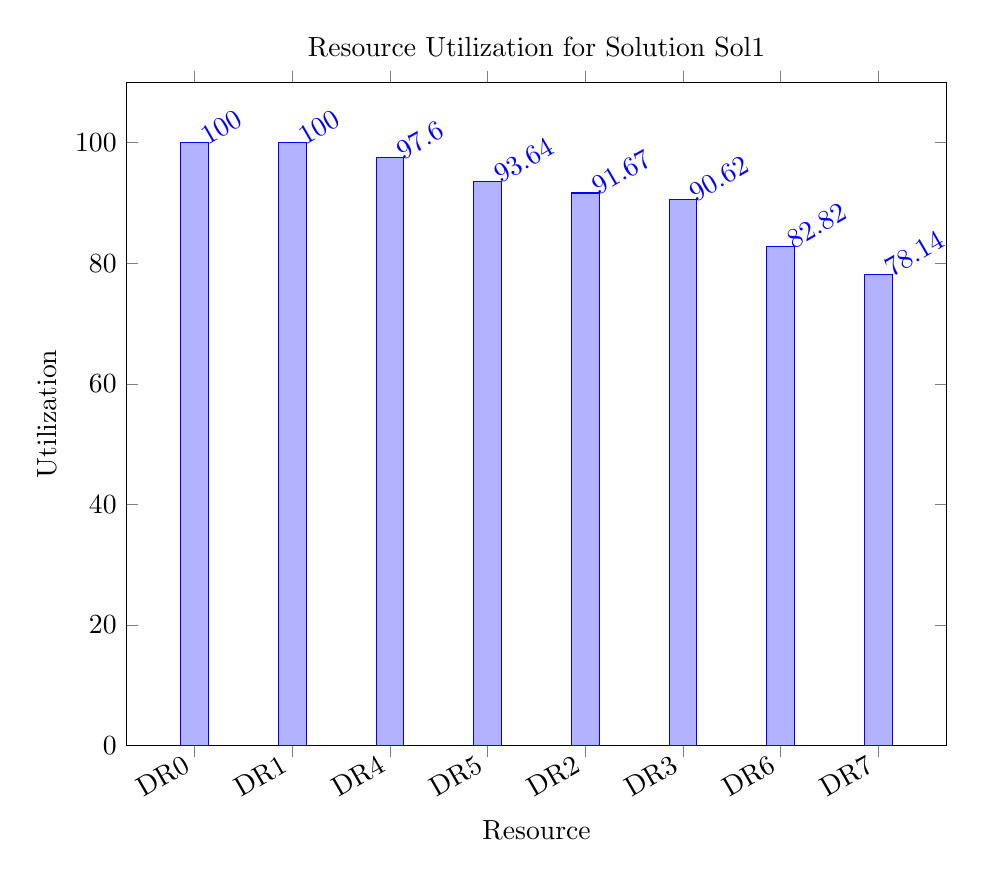
\begin{tikzpicture}
\begin{axis}[title=Resource Utilization for Solution Sol1,xlabel=Resource,ylabel=Utilization,ymin=0,
width=12cm,height=10cm,ybar,
symbolic x coords={DR0,DR1,DR4,DR5,DR2,DR3,DR6,DR7},
    xtick=data,nodes near coords, nodes near coords align={rotate=30),anchor=west},x tick label style={rotate=30),anchor=east}]
\addplot+[] coordinates {
(DR0,100.000000)
(DR1,100.000000)
(DR4,97.597977)
(DR5,93.636364)
(DR2,91.666667)
(DR3,90.620872)
(DR6,82.815057)
(DR7,78.144654)
};
\end{axis}
\end{tikzpicture}

\begin{tikzpicture}
\begin{axis}[title=Cumulative Resource Use CR0,xlabel=Time,ylabel=Resource Use,enlarge x limits=0.01,no markers,,legend pos=outer north east,xmin=0,xmax=903,width=21cm,height=12cm]
\addplot+ [const plot] coordinates {
    (0,10)
    (903,0)
    (903,0)
};
\addlegendentry{Capacity}
\addplot+ [const plot] coordinates {
    (0,2)
    (54,3)
    (63,4)
    (126,5)
    (155,6)
    (198,5)
    (255,6)
    (311,7)
    (315,8)
    (333,7)
    (360,6)
    (381,5)
    (383,6)
    (414,7)
    (441,8)
    (517,7)
    (524,8)
    (548,7)
    (561,6)
    (577,7)
    (592,8)
    (628,7)
    (714,6)
    (731,5)
    (739,6)
    (762,5)
    (801,4)
    (807,5)
    (813,4)
    (815,5)
    (820,4)
    (884,3)
    (888,2)
    (902,1)
    (903,0)
    (903,0)
};
\addlegendentry{Demand}
\end{axis}
\end{tikzpicture}

\end{document}
